%The KUCC algorithm leverage the OOT pulse amplitudes determined by the multi-fit algorithm for the rechit energy reconstruction for use in the timing reconstruction.  Given these amplitudes and the known pulse shape of an isolated signal in a crystal, we reconstruct the nominal pulse contribution from the measured amplitudes for a rechit. By extracting the nominal pulse to use in reconstruction of the rechit time and finding the time via the cross correlation function that best matches the extracted signal amplitudes to the pulse shape template, we significantly mitigate the effect of OOT PU and improve the ECAL time resolution. 

%The plot of the mean rechit time by BX position for a typical BX train, as shown in section \ref{sec:reco4}, was produced using the KUCC rechit collection. This plot, as seen in Figure~\ref{cclhcplots1}, illustrate the cross correlation methods ability to mitigate the effect of OOT pile-up. 
%As discussed in Section \ref{sec:reco4}, 
OOT-PU occurs when interactions from particles originating in events from BXs before the current BX are seen in events recorded during the current BX. In particular, signals produced by scintillating light pulses in ECAL crystals are longer than 25 ns, the nominal time between BXs.  This can easily result in signals produce by particles originating in different BXs overlapping and impacting the time reconstruction. The effect of OOT-PU on the time reconstruction can be seen when the mean rechit time by BX position in the "train" of filled BXs is studied. 

\hfill
\begin{figure}[h!tbp]
\begin{center}
%\resizebox{0.5\textwidth}{!}{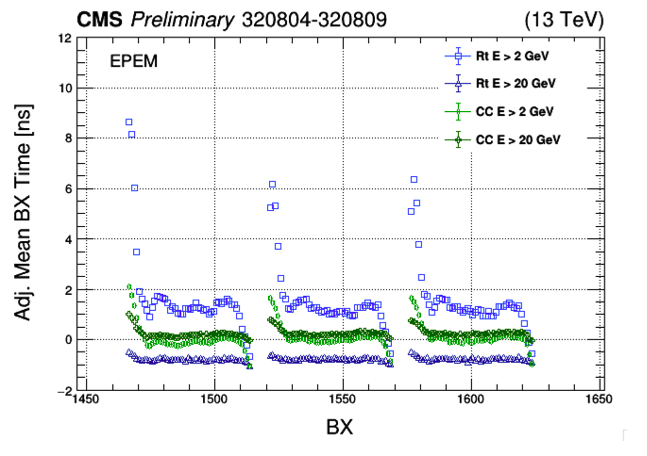
\includegraphics{fig/sec_results/lhc_cc_v_rt_plot.png}}
\resizebox{0.7\textwidth}{!}{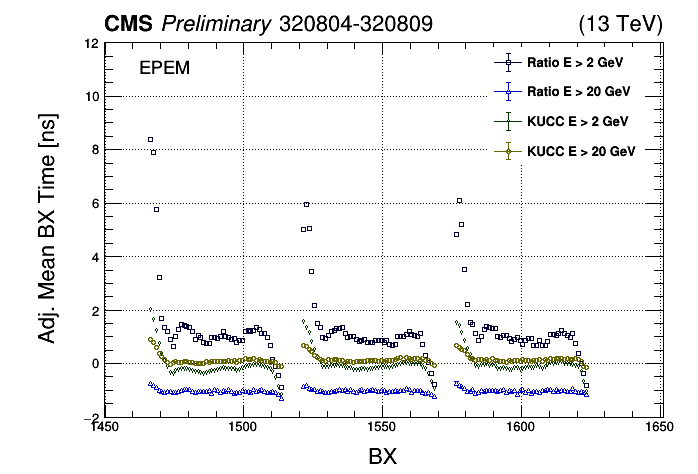
\includegraphics{fig/sec_results/tr_lhc_18A_v25_talk_30112021151421.png}}
\caption{Mean rechit time by BX, for rechits with a minimum of 2 GeV ( 20 GeV ) with both the ratio and CC reconstructions, for a typical train of filled buckets is plotted. The plotted values are adjusted so that the mean rechit time by BX when averaged over all BXs and energies is zero. The CC algorithm is shown to mitigate the impact of OOT-PU through the reduced dependence of the time on the BX position and to achieve a greatly reduced energy dependence.}
% in Runs 320804 through 320809 of EGamma Run2018D-22Jan2019-v2
\label{cclhcplots1}
\end{center}
\end{figure}

In Figure~\ref{cclhcplots1} the mean rechit time by BX for rechits with a minimum of 2 GeV, and for rechits with a minimum of 20 GeV, for rechit collections produced with the default ratio algorithm and the CC algorithm are plotted. For this plot the rechit times are calibrated by subtracting the mean time across all BXs for rechits with a minimum of 5 GeV in the corresponding rechit collection. It can be seen in the leading and trailing tails of the trains that the CC algorithm significantly reduces dependence of the rechit time on the BX position and therefore mitigates the impact of OOT-PU on the reconstruction. The central regions of the sub-trains exhibit a markedly reduce spread between the 2 GeV and 20 GeV data points for the CC algorithm compared to the ratio algorithm indicating that the CC algorithm produces a greatly reduce energy dependence in the time reconstruction.
 % for Runs 320804 through 320809 in EGamma Run2018D-22Jan2019-v2 rereco. 
 
%begin{figure}[h!tbp]
%\begin{center}
%\resizebox{0.5\textwidth}{!}{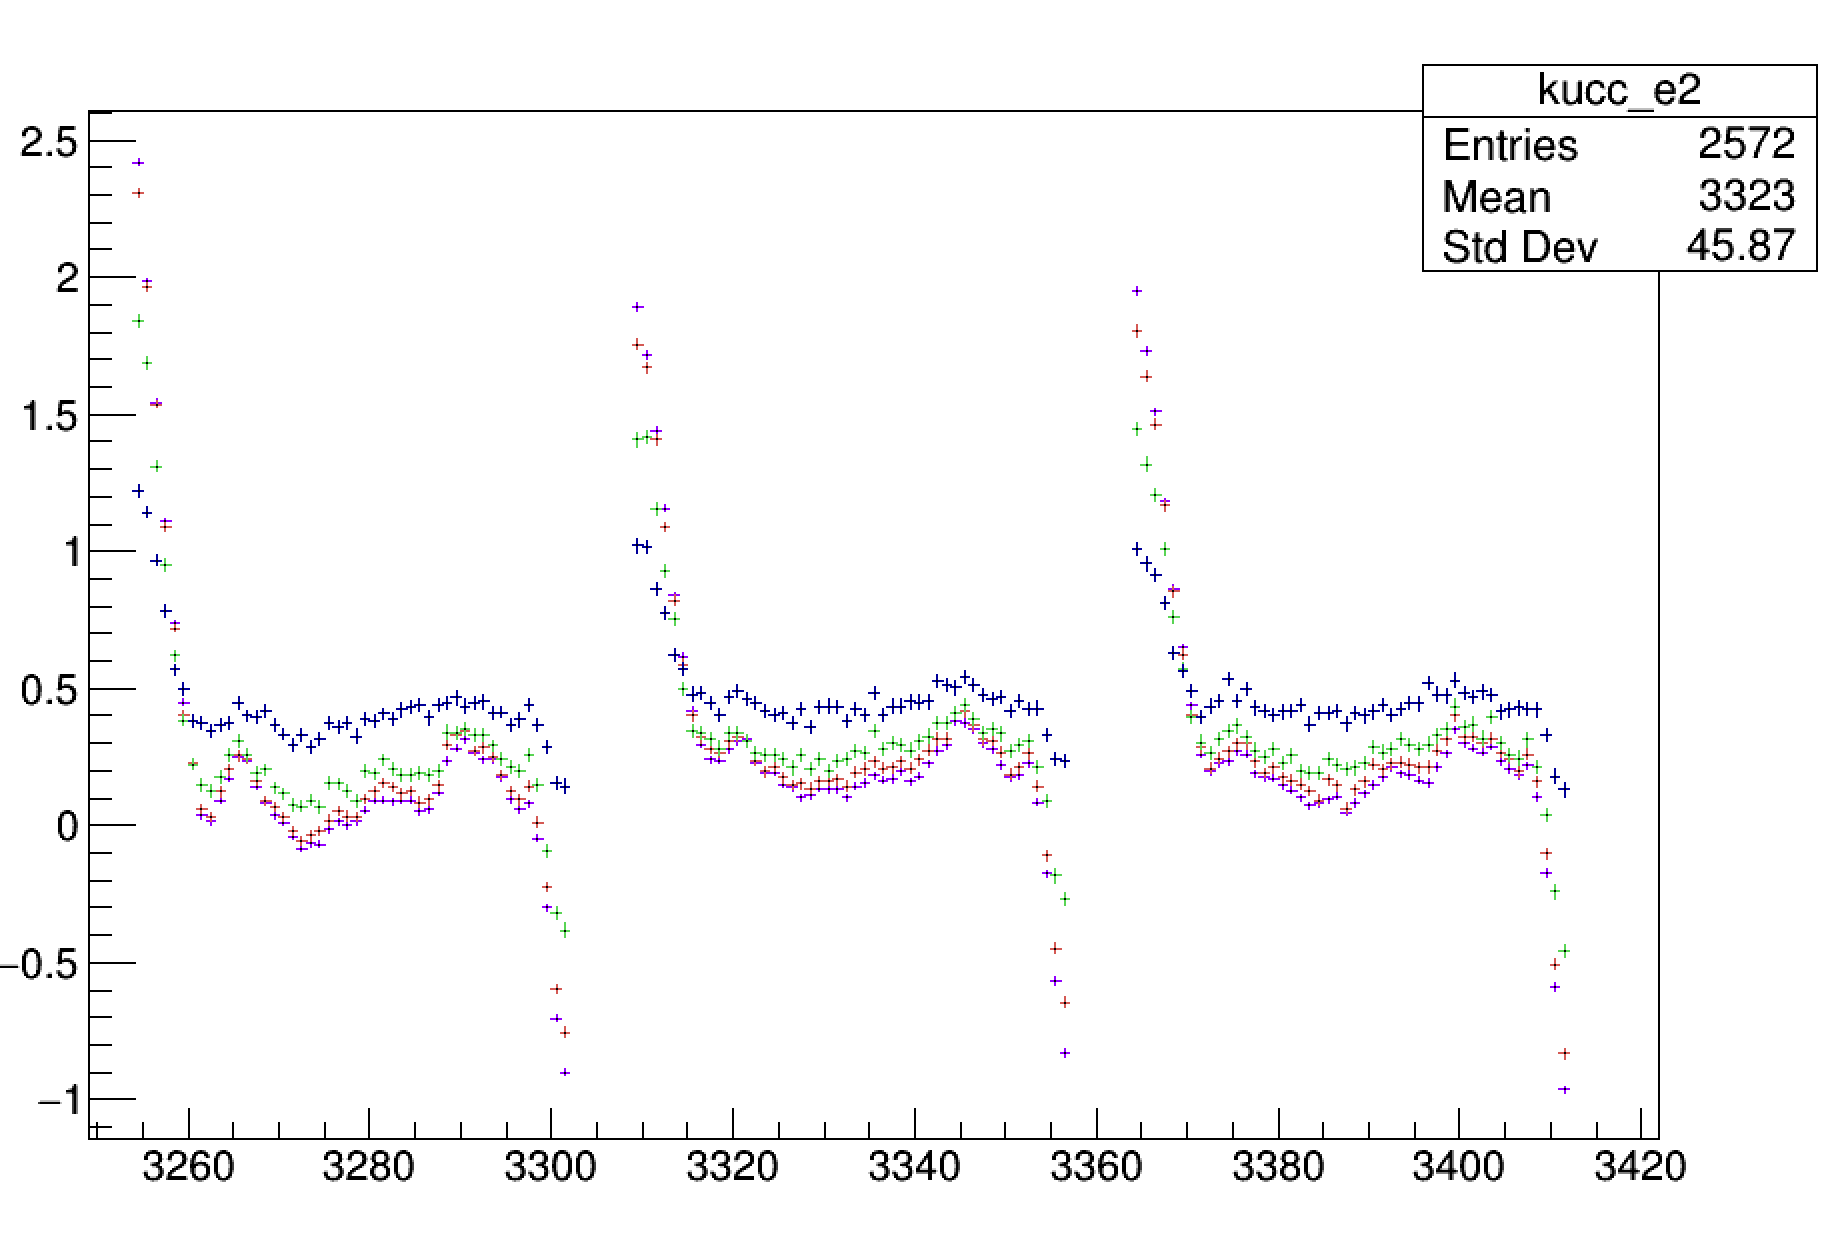
\includegraphics{fig/sec_results/lhcinfo_cc_prelim.png}}
%\caption{  ..  lhcinfo with cc - replace plot with pretty version ...}
%\label{cclhcplots2}
%\end{center}
%\end{figure}

\hfill
\begin{figure}[h!tbp]
\begin{center}
%\resizebox{0.5\textwidth}{!}{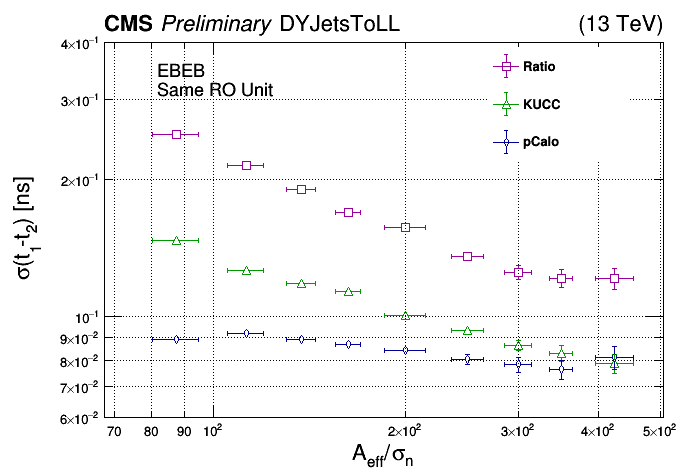
\includegraphics{fig/sec_gen/tr_mc_pc2_loc_plot_07122020164223.png}}
\resizebox{0.7\textwidth}{!}{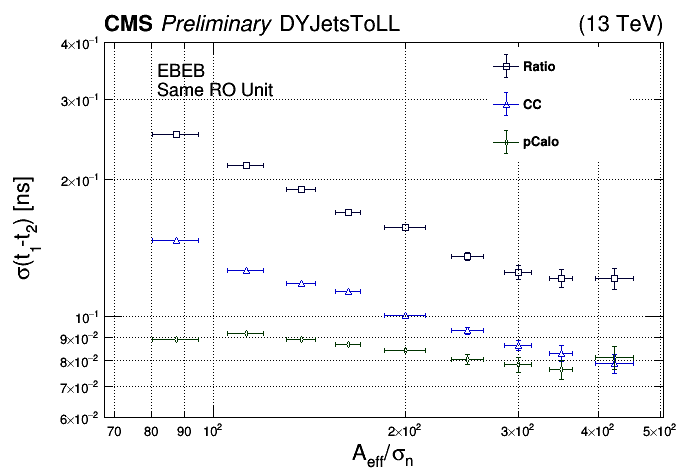
\includegraphics{fig/sec_gen/tr_mc_pc2_loc_plot_30112021153817.png}}
\caption{Same RO unit, single crystal resolutions for the ratio algorithm, the CC algorithm, and pCaloHit gen time are compared in simulation.  The CC algorithm shows a much improved resolution compared to the ratio algorithm and approaches the pCaloHit gen time resolution at high energies.}
%produced with the DYJetsToLL\_M-50\_TuneCP5\_13TeV-madgraphMLM-pythia8 Monte Carlo dataset.
\label{pc_rt_cc_comp}
\end{center}
\end{figure}

During development, time using the CC algorithm for the time reconstruction were produced using a two tier processing approach. This allows for both the time produced with the CC time reconstruction and the already existing time from the ratio time reconstruction to be recorded for each rechit. With this information the performance of the two algorithms can be directly compared. Studies comparing the performance of the CC and ratio time reconstruction were done in both simulation ( MC ) and recorded data.
%With this approach the CC rechit collection was produced while processing data in the miniAOD format from the parent RAW data stream of the miniAOD data.
%In Figure~\ref{tra_tdist} a typical time distribution from for the leading photon used in a local time resolution using the KUCC time algorithm is shown.
%The standard method for determine the time resolution was preformed with the rechit collection produced using the KUCC timing algorithm. 

%\begin{figure}[h!tbp]
%\begin{center}
%\resizebox{0.4\linewidth}{!}{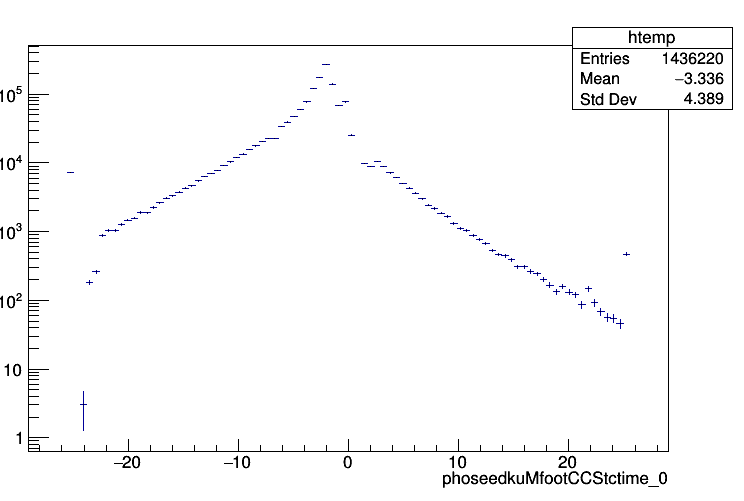
\includegraphics{fig/sec_algos/cc_dist_temp.png}}
%\caption{Typical time distribution in a photon produced by the cross-correlation time reconstruction method.  }
%\label{tra_tdist}
%\end{center}
%\end{figure}

\hfill
\begin{figure}[h!tbp]
\begin{center}
%\resizebox{0.33\textwidth}{!}{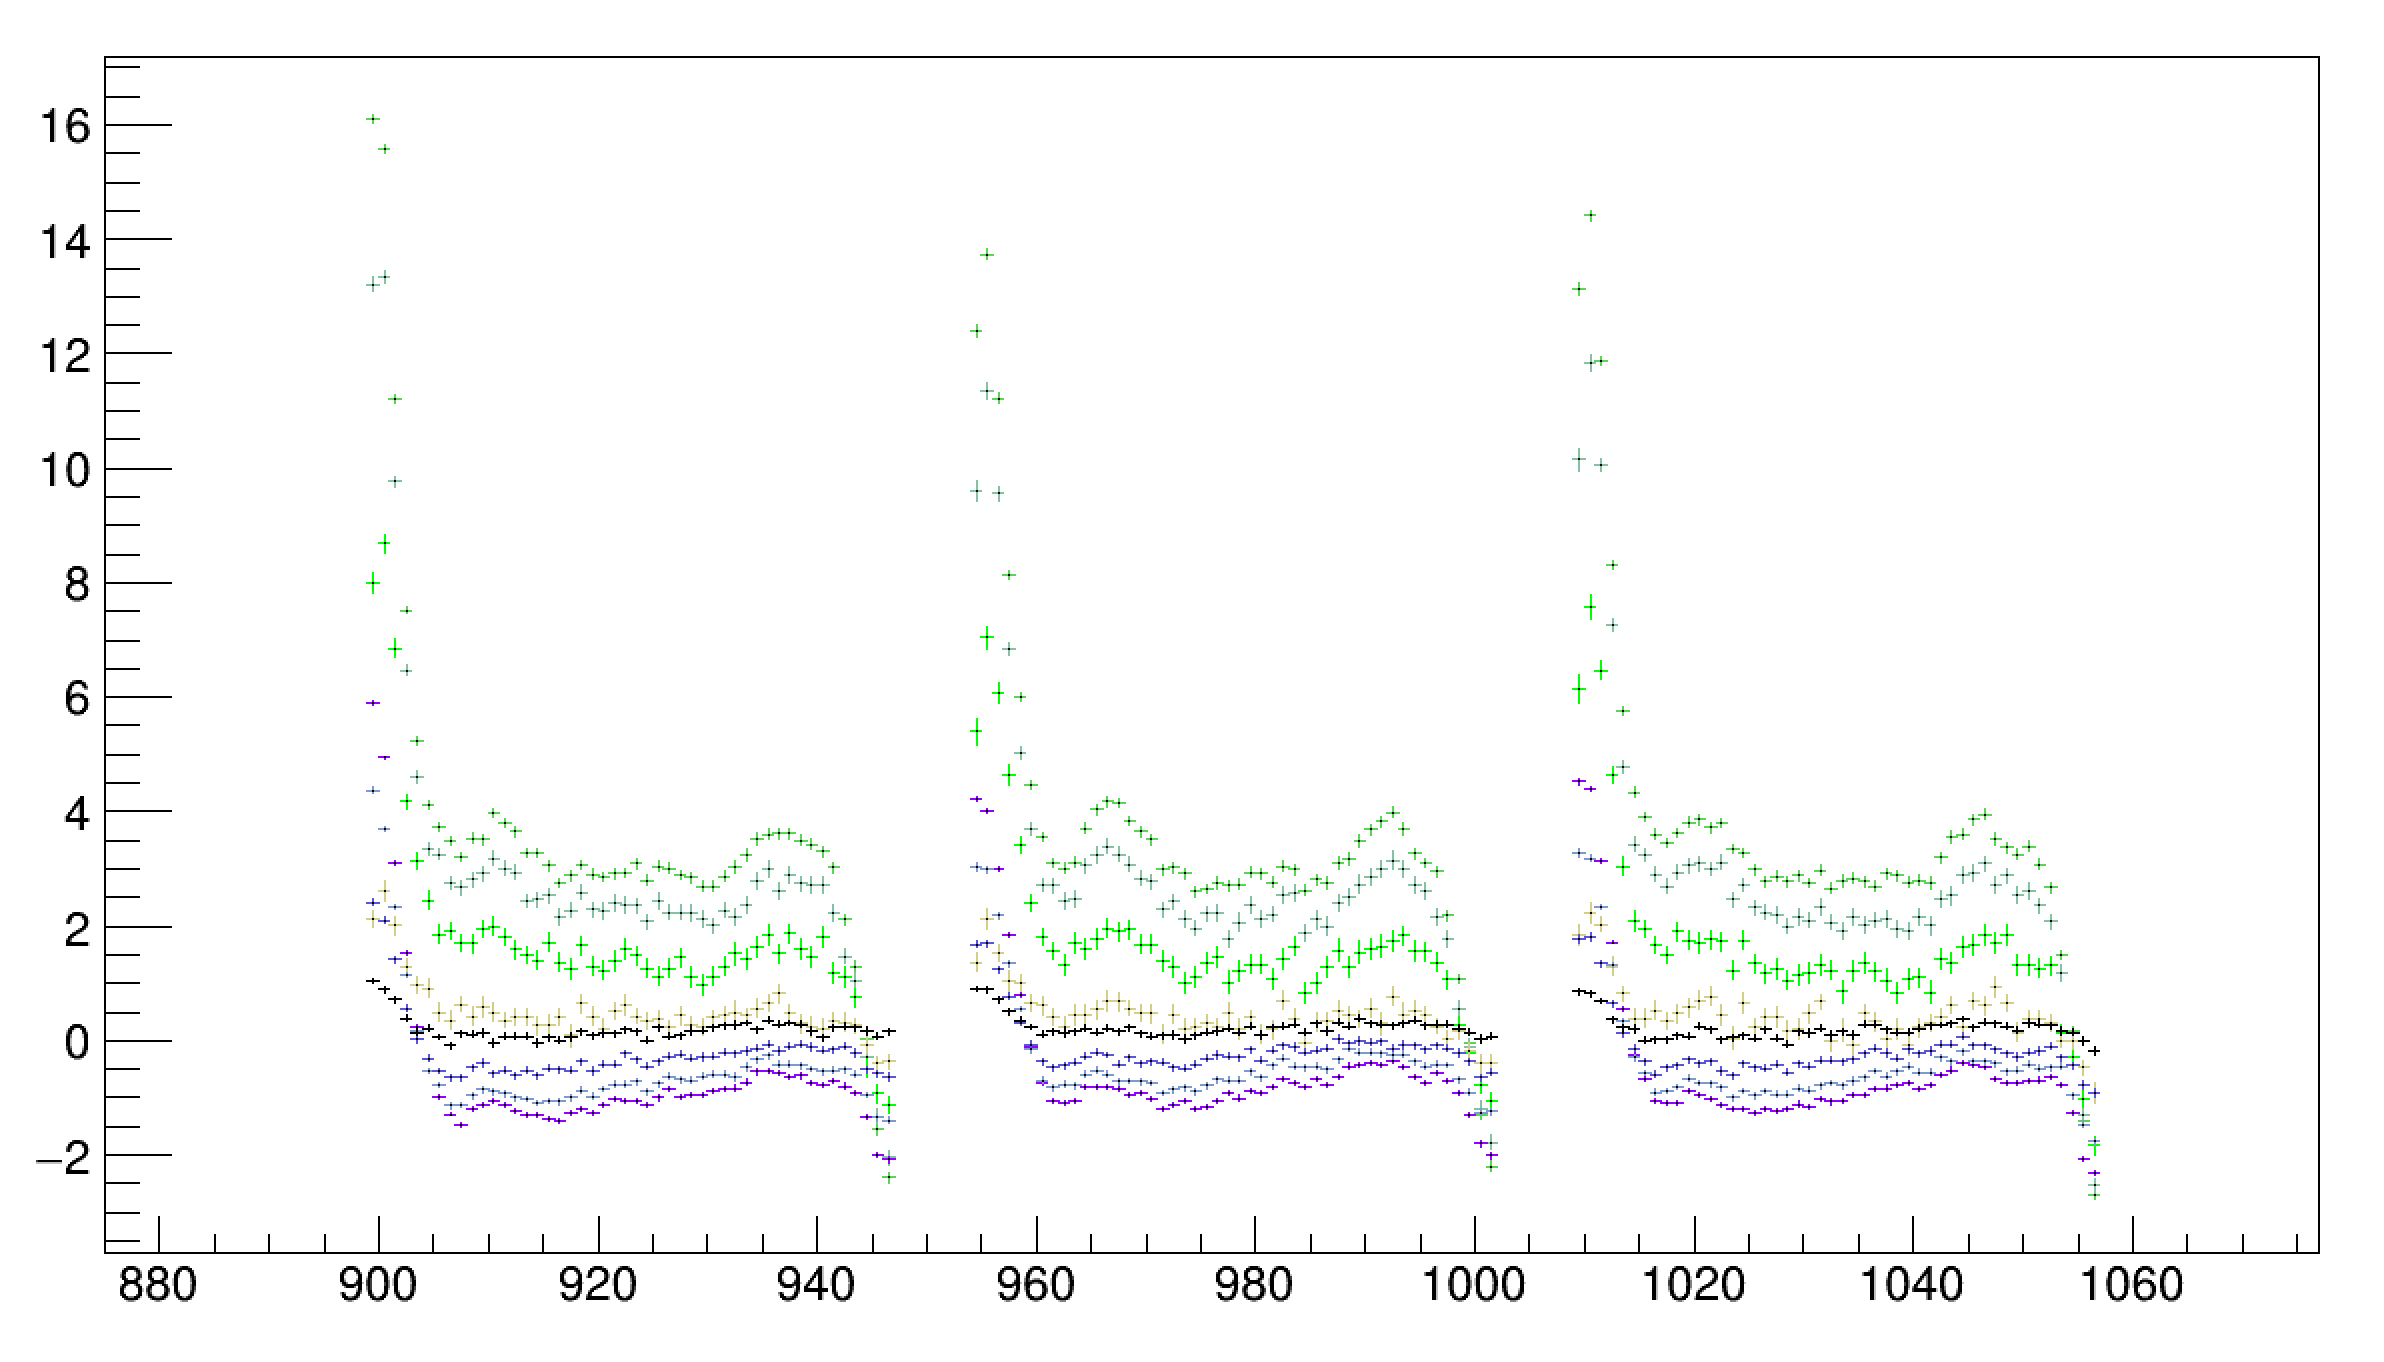
\includegraphics{fig/sec_results/full_lhc_info.png}}
%\resizebox{0.5\textwidth}{!}{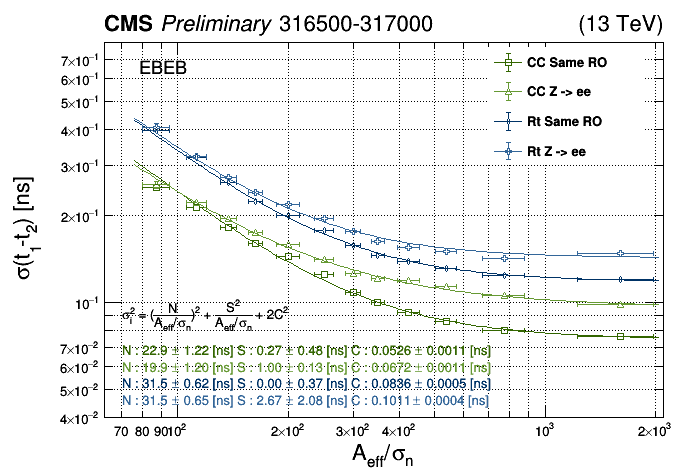
\includegraphics{fig/sec_results/tr_kucc_18As_v25_talk_17092021152333.png}}
\resizebox{0.7\textwidth}{!}{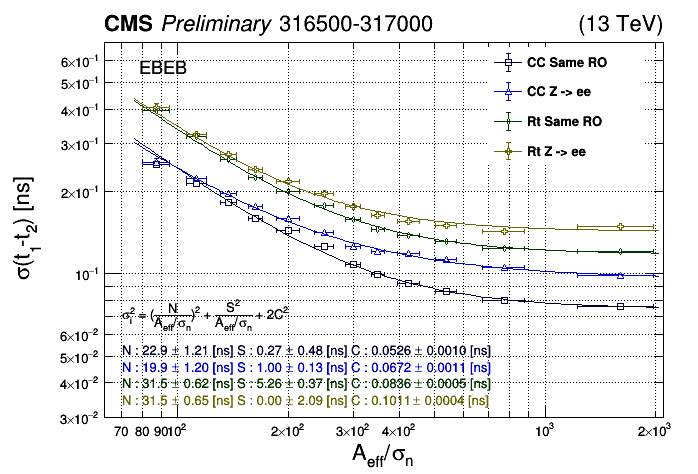
\includegraphics{fig/sec_results/tr_kucc_18As_v25_talk_30112021160215.png}}
\caption{Comparison of time Same RO and $Z\rightarrow e^{+}e^{-}$ resolution for CC and the ratio algorithms in Run 2 using the two tier data processing approach and external calibrations. This plot shows that the CC algorithms achieves an improvement in the Same RO unit resolution of $\sim$30 ps and an $Z\rightarrow e^{+}e^{-}$ resolution improvement of $\sim$35 ps.}
%\caption{Comparison of time Same RO and $Z\rightarrow e^{+}e^{-}$ resolution for KUCC and the ratio algorithms in run 316500 through run 317000 of the EGamma Run2018A-17Sep2018-v2 rereco. This plot shows that the CC algorithms achieves an improvement in the Same RO unit resolution of $\sim$30 ps and an $Z\rightarrow e^{+}e^{-}$ resolution improvement of $\sim$35 ps.}
\label{ccresr2}
\end{center}
\end{figure}

The resolution obtained by the CC algorithm in MC were studied in comparison to both the ratio algorithm and to pCalo gen times. these studies where performed with Run 2 MC using the two tier data processing approach and an external calibration. Since, as noted in section~\ref{sec:resmeth2}, for MC the data used as input for the timing reconstruction methods is derived from the pCaloHit collection. Therefore, the resolution obtained using the pCaloHit gen time reference is a reasonable estimate of the best resolution achievable by a timing reconstruction method. In Figure~\ref{pc_rt_cc_comp} the single crystal resolutions for the ratio algorithm, the CC algorithm, and pCalo gen time are plotted. It is seen here that the resolution of the CC algorithm is significantly narrower than the resolution of the ratio algorithm across all effective amplitudes and at larger effective amplitudes the resolution of the CC algorithm approaches the pCalo gen time resolution.   
% in DYJetsToLL\_M-50. 

\hfill
\begin{figure}[h!tbp]
\begin{center}
%\resizebox{0.33\textwidth}{!}{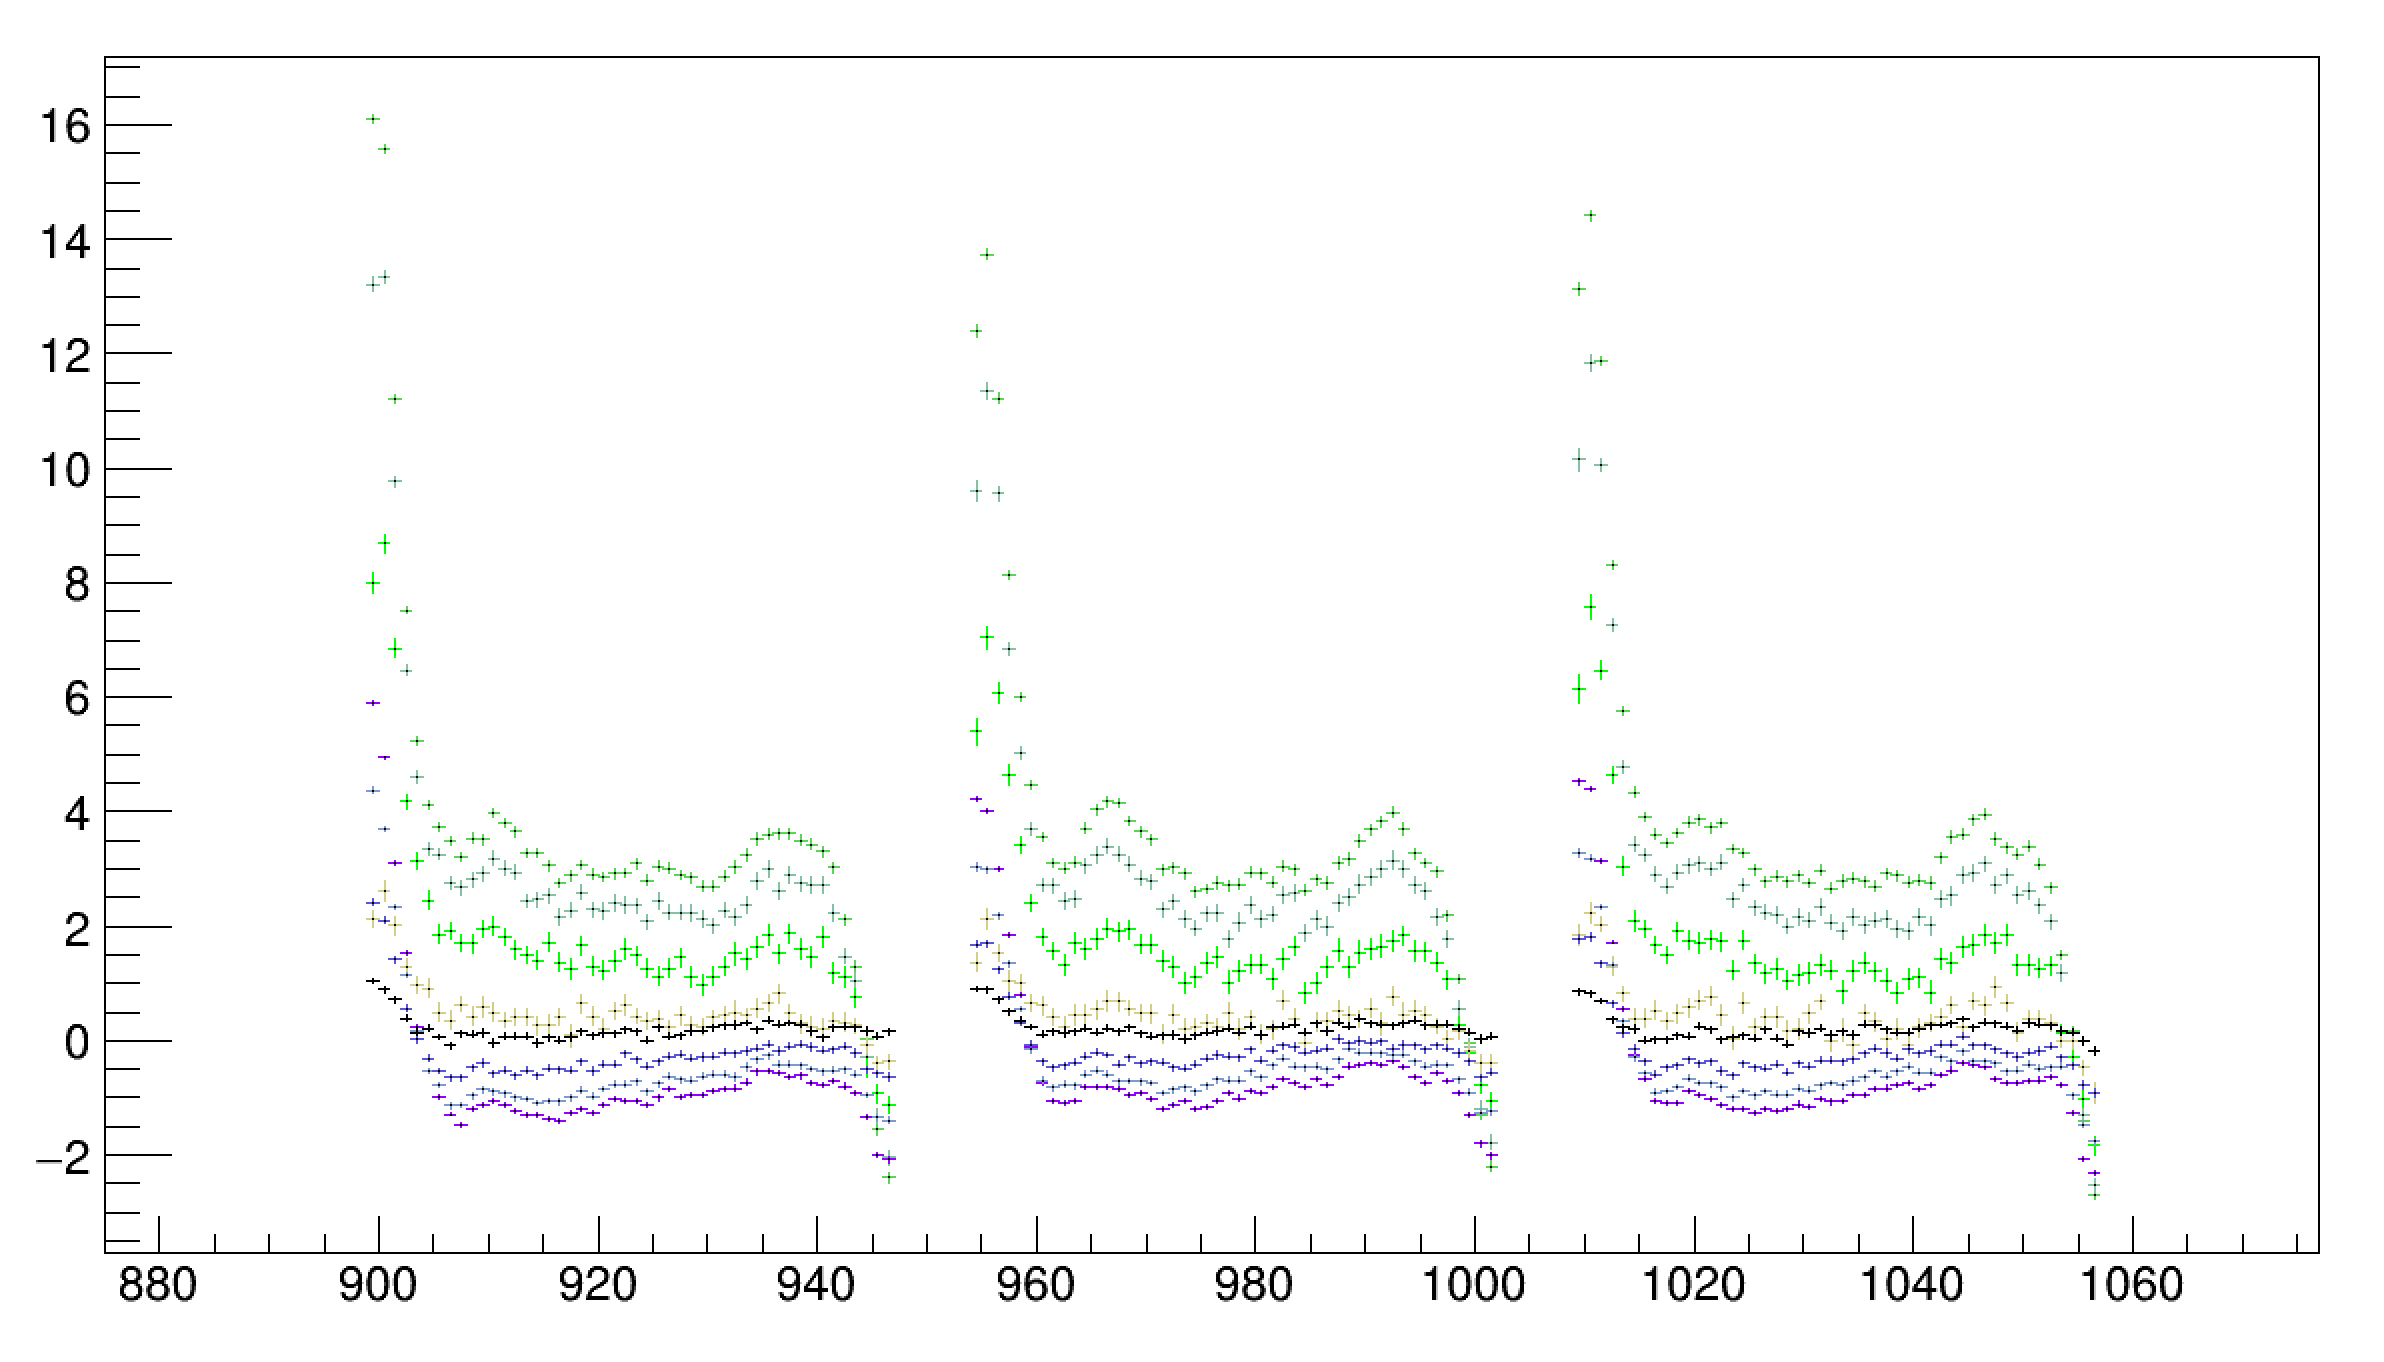
\includegraphics{fig/sec_results/full_lhc_info.png}}
%\resizebox{0.5\textwidth}{!}{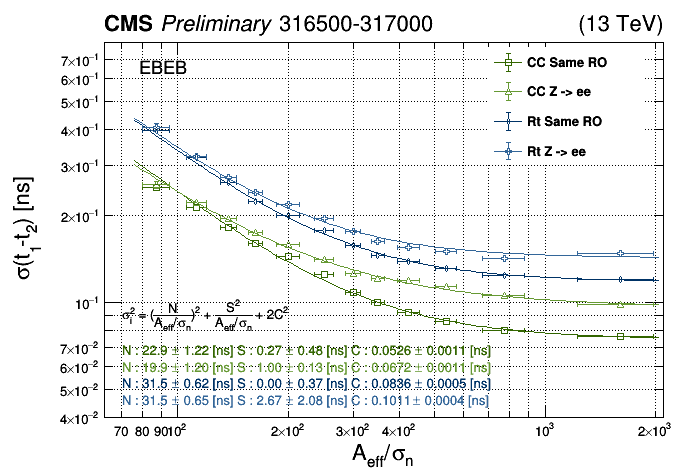
\includegraphics{fig/sec_results/tr_kucc_18As_v25_talk_17092021152333.png}}
\resizebox{0.7\textwidth}{!}{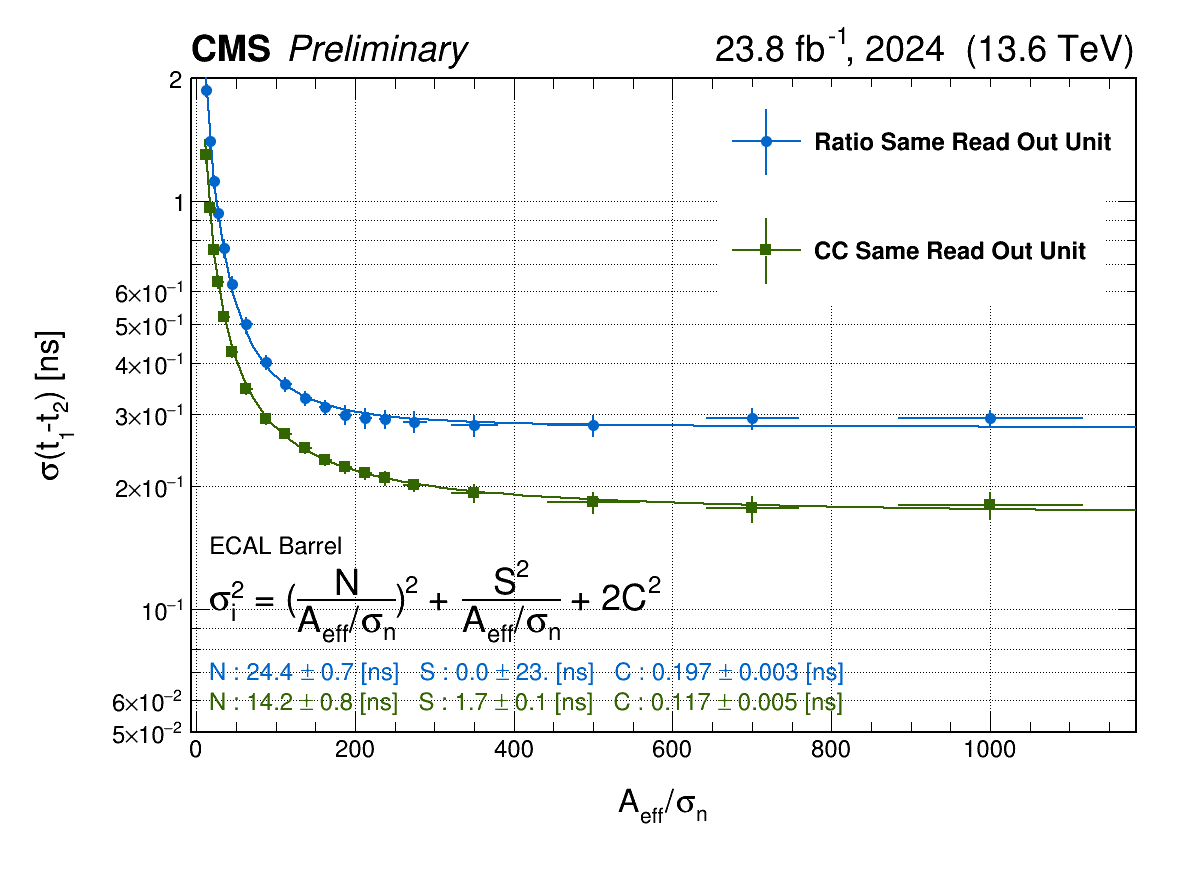
\includegraphics{fig/sec_results/tr_hl_r3_24f_v2_rtvcc_xgs_07082025170637.png}}
\caption{Comparison of time Same RO and $Z\rightarrow e^{+}e^{-}$ resolution for CC and the ratio algorithms in Run 3. In Run 3 the CC algorithm had been implemented in CMSSW and a dedicated online calibration was implemented. This plot shows the comparative resolutions obtained from two separate full prompt reconstructions of the same data where the ratio was default for one of the reconstructions and the CC method was the default for the other reconstruction. This plot shows that the CC algorithms achieves an improvement in the Same RO unit resolution of $\sim$ 80 ps.}
%\caption{Comparison of time Same RO and $Z\rightarrow e^{+}e^{-}$ resolution for CC and the ratio algorithms in run 316500 through run 317000 of the EGamma Run2018A-17Sep2018-v2 rereco. This plot shows that the KUCC algorithms achieves an improvement in the Same RO unit resolution of $\sim$30 ps and an $Z\rightarrow e^{+}e^{-}$ resolution improvement of $\sim$35 ps.}
\label{ccresr3}
\end{center}
\end{figure}

%**************** Show an example plot of CC time distribution ?
%In Figure~\ref{ccdistros} the distribution of the cross correlation rechit times from the crystals selected for a local resolution are shown on the left and 2D plot of the $\Delta(t_{0}-t_{1})$ with respect to the effective amplitude is shown on the right. 
%Direct comparison of the resolution obtained with the CC algorithm compared with the ratio algorithm was studied in data. 
Figure~\ref{ccresr2} shows the same readout unit and $Z\rightarrow e^{+}e^{-}$ resolution in Run 2 using the two tier data processing approach and external calibrations for recorded data. The CC algorithm produces an improvement $\sim$30 ps for the same RO unit resolution and an improvement of $\sim$35 ps for the $Z\rightarrow e^{+}e^{-}$ resolution compared to the ratio algorithm reconstruction.  In Figure~\ref{ccresr3} resolutions obtained in Run 3 are studied.  During Run 3 the CC algorithm was implemented in CMSSW and a dedicated online calibration was implemented. This plot shows the comparative resolutions obtained from two separate full prompt reconstructions of the same data where the ratio was default for one of the reconstructions and the CC method was the default for the other reconstruction. Here we see that the CC algorithms achieves an improvement in the Same RO unit resolution of $\sim$ 80 ps. The CC time reconstruction was the default time reconstruction used for data taking in 2025 of Run 3.  In Figure~\ref{ccresr4} we see the same readout unit and $Z\rightarrow e^{+}e^{-}$ resolutions obtained by the CC reconstruction during the first data taking period with sufficient statistics for a resolution study in 2025. The CC algorithms achieves a Same RO unit resolution of $\sim$ 135 ps and a $Z\rightarrow e^{+}e^{-}$ resolution of $\sim$ 180 ps. Comparing the $Z\rightarrow e^{+}e^{-}$ resolution of $\sim$ 180 ps achieved by the CC time reconstruction to the Same RO unit resolution of $\sim$ 200 ps achieved by the ratio time reconstruction, as seen in Figure~\ref{ccresr3}, we can deduce that the CC time reconstruction significantly midgets the impact of OOT-PU on the time reconstruction.

%in a prompt reconstruction from data in 2025 during Run 3.
%The CC algorithm is expected to achieve $Z\rightarrow e^{+}e^{-}$, analysis relevant E/gamma object, resolutions of $\sim$100 ps to $\sim$200 ps, compared to $\sim$300 ps typical in Run II. With the utilization of the CC algorithm we expect comparable, if not improved, resolutions for Run III.

%Direct comparison of the resolution obtained with the CC algorithm compared with the ratio algorithm was studied in data. Figure~\ref{ccres} shows the same readout unit and $Z\rightarrow e^{+}e^{-}$ resolution plotted over EGamma 2018A data stream for runs 316241 to 316457. The KUCC algorithm produces an improvement $\sim$30 ps for the same RO unit resolution and an improvement of $\sim$35 ps for the $Z\rightarrow e^{+}e^{-}$ resolution compared to the ratio algorithm reconstruction. The CC algorithm is expected to achieve $Z\rightarrow e^{+}e^{-}$, analysis relevant E/gamma object, resolutions of $\sim$100 ps, compared to $\sim$300 ps typical in Run II. With the utilization of the CC algorithm we expect comparable, if not improved, resolutions in Run III.

\hfill
\begin{figure}[h!tbp]
\begin{center}
%\resizebox{0.33\textwidth}{!}{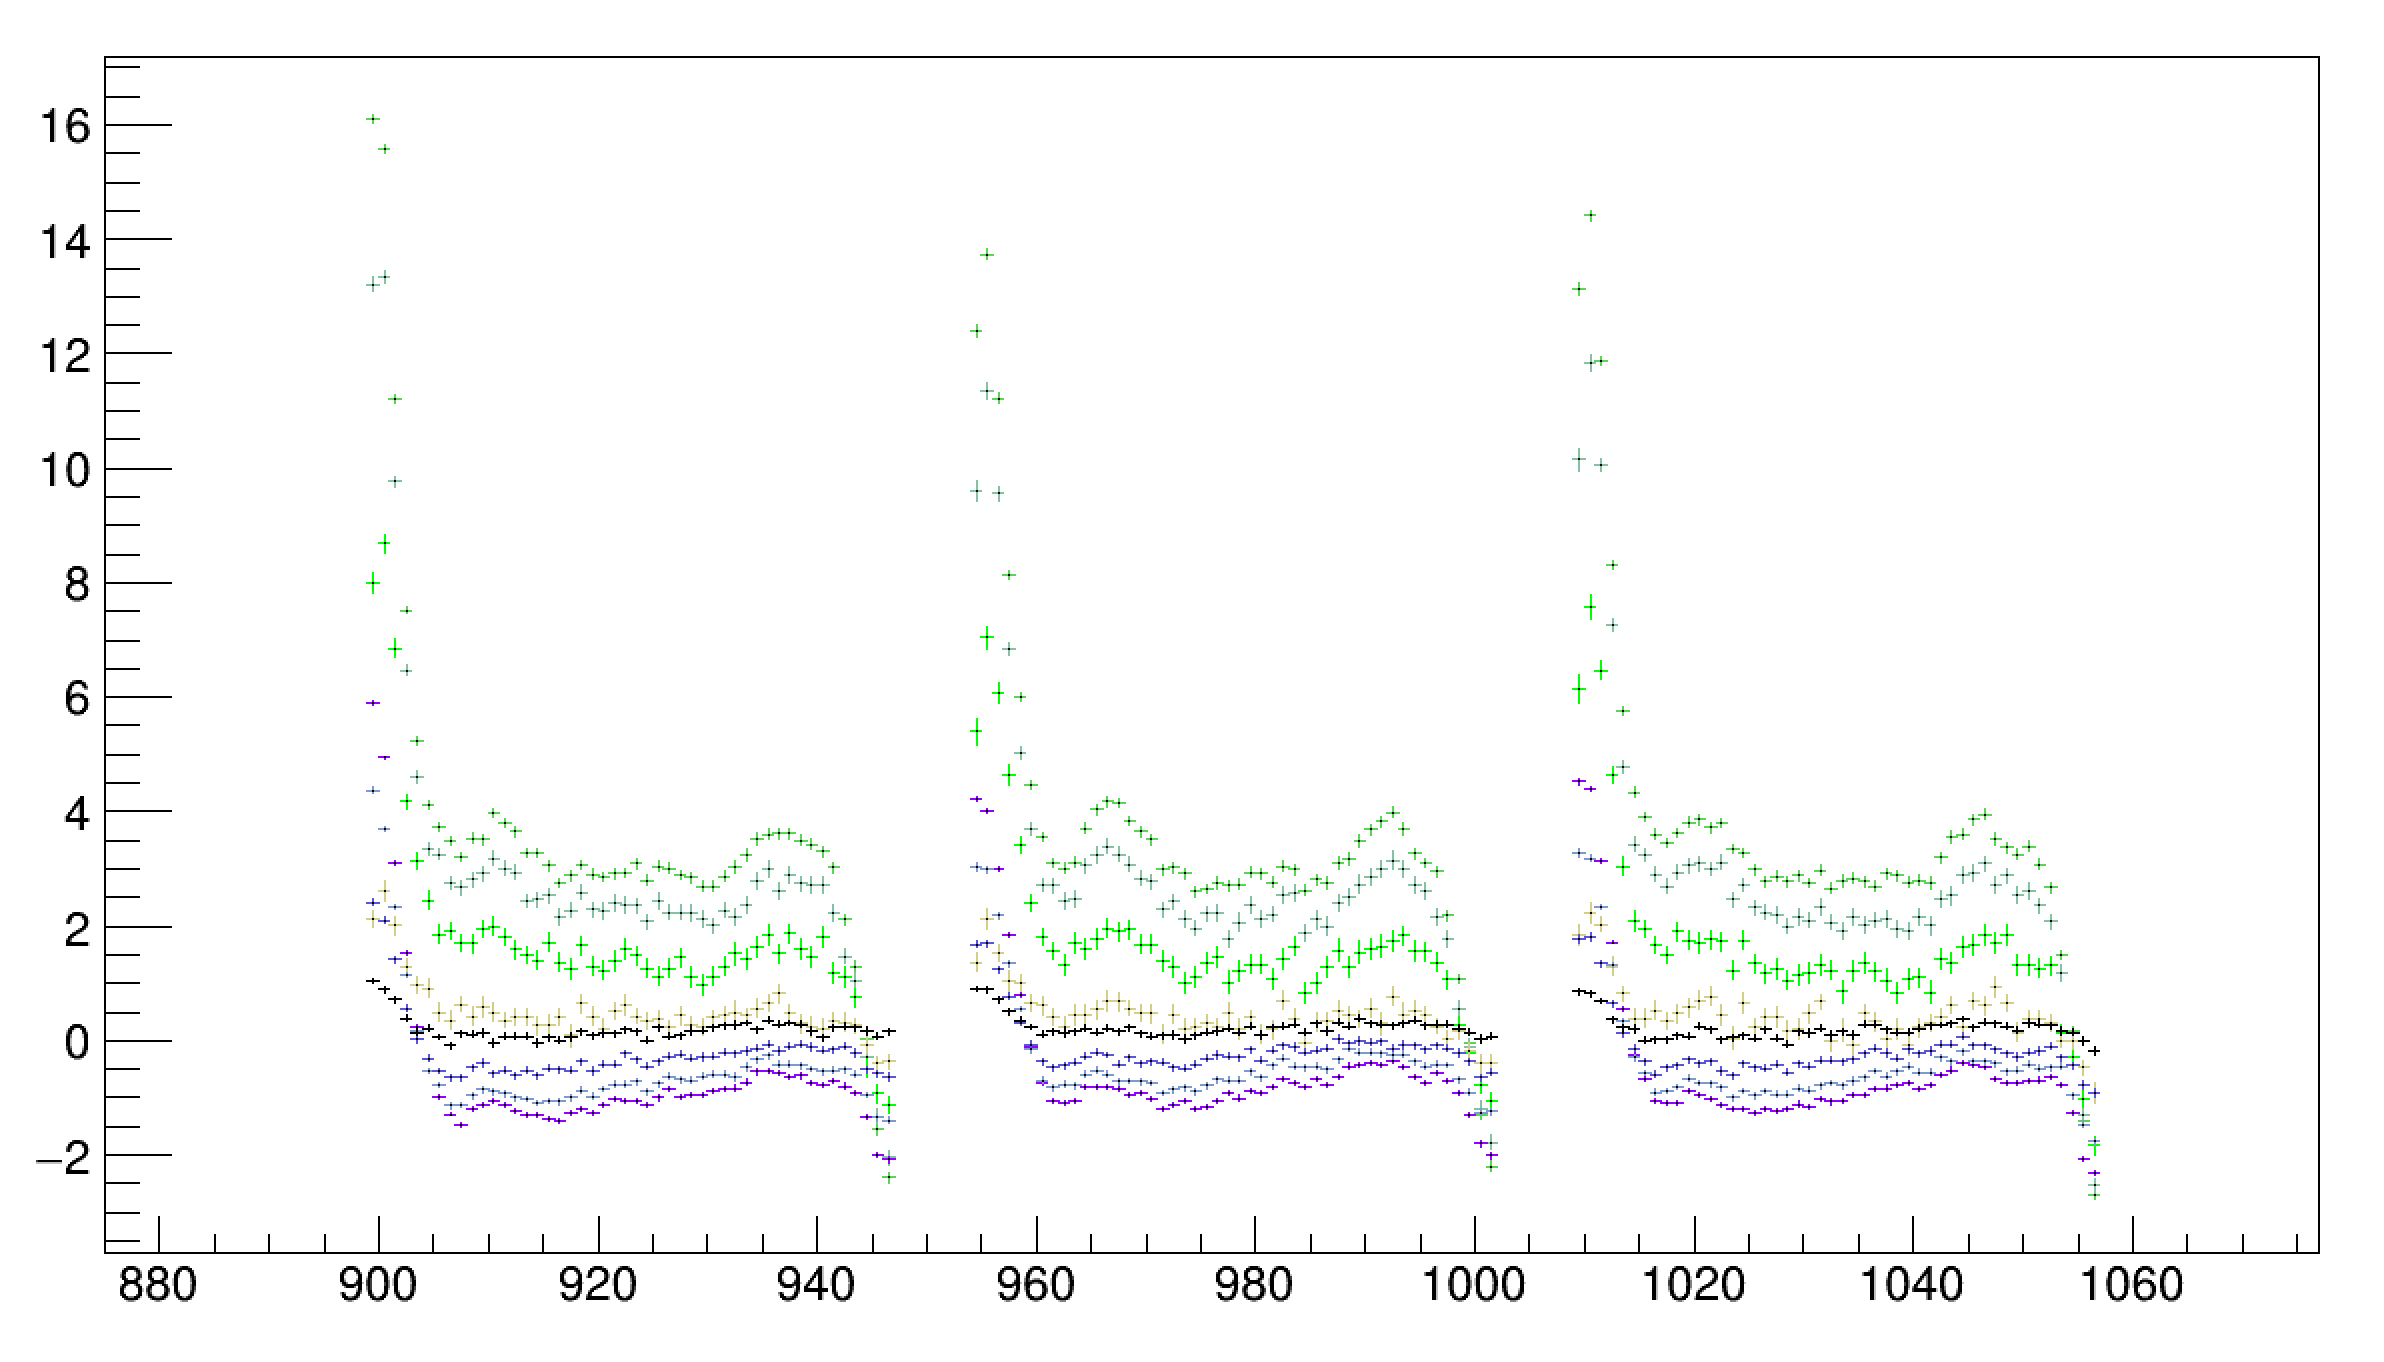
\includegraphics{fig/sec_results/full_lhc_info.png}}
%\resizebox{0.5\textwidth}{!}{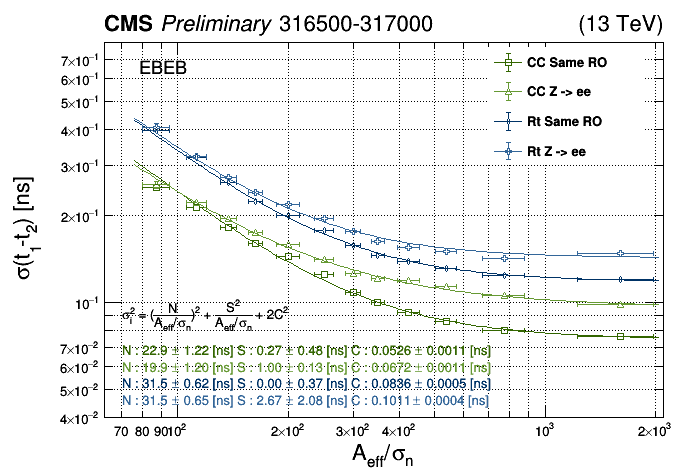
\includegraphics{fig/sec_results/tr_kucc_18As_v25_talk_17092021152333.png}}
\resizebox{0.7\textwidth}{!}{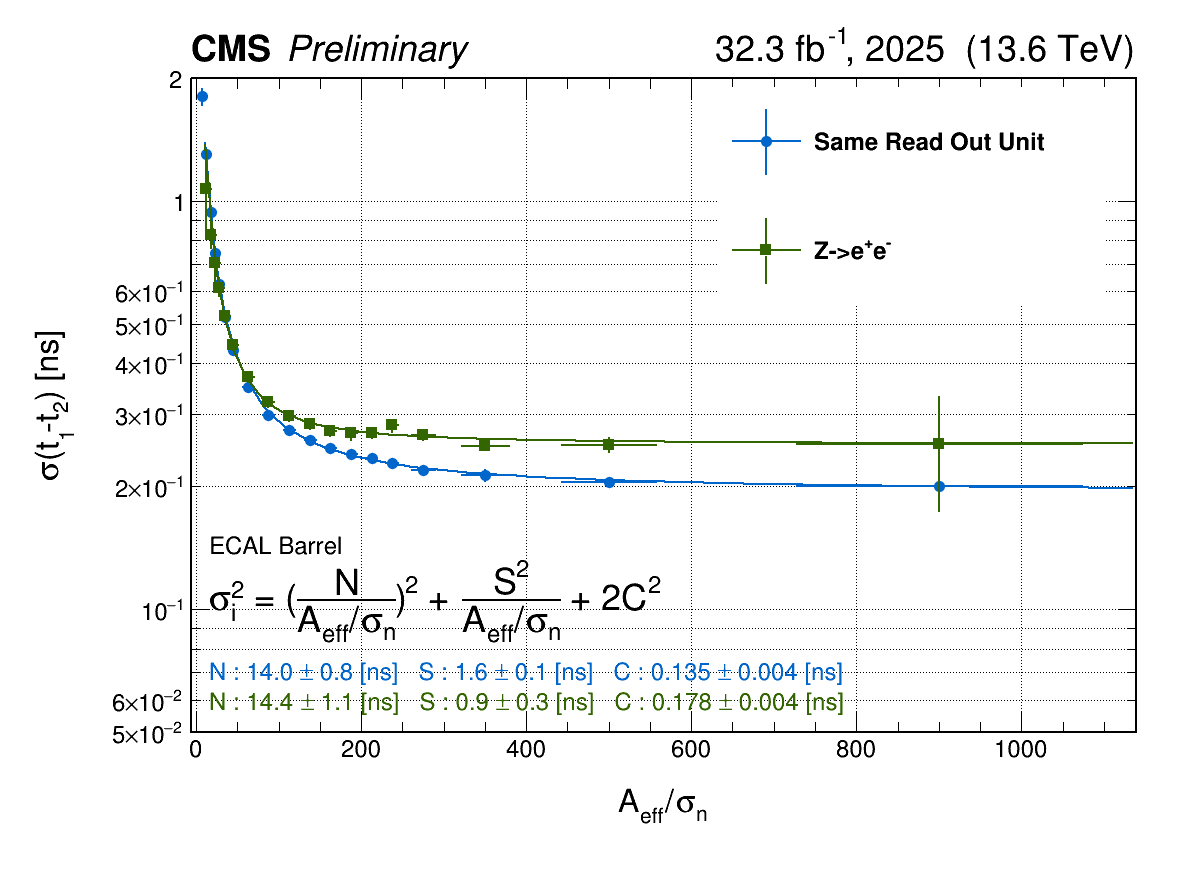
\includegraphics{fig/sec_results/tr_hl_r3_25c2_08082025165318.png}}
\caption{Same RO and $Z\rightarrow e^{+}e^{-}$ resolution for CC in Run 3. The CC algorithm, along with a dedicated online calibration, was implemented in CMSSW in 2024 of Run 3 and was the default ECAL time reconstruction in 2025. This plot shows the Same RO and $Z\rightarrow e^{+}e^{-}$ resolutions for obtained during a prompt reconstruction with the CC method. Here we see that the CC algorithms achieves a Same RO unit resolution of $\sim$ 135 ps and an $Z\rightarrow e^{+}e^{-}$ resolution of $\sim$ 180 ps in prompt reconstruction.}
%\caption{Comparison of time Same RO and $Z\rightarrow e^{+}e^{-}$ resolution for CC and the ratio algorithms in run 316500 through run 317000 of the EGamma Run2018A-17Sep2018-v2 rereco. This plot shows that the KUCC algorithms achieves an improvement in the Same RO unit resolution of $\sim$30 ps and an $Z\rightarrow e^{+}e^{-}$ resolution improvement of $\sim$35 ps.}
\label{ccresr4}
\end{center}
\end{figure}



%\begin{figure}[htbp]
%\begin{center}
%\resizebox{0.33\textwidth}{!}{\inculudegraphics{fig/sec_algos/dt_effa_v24_18A_316241_316457.pdf}}
%\resizebox{0.33\textwidth}{!}{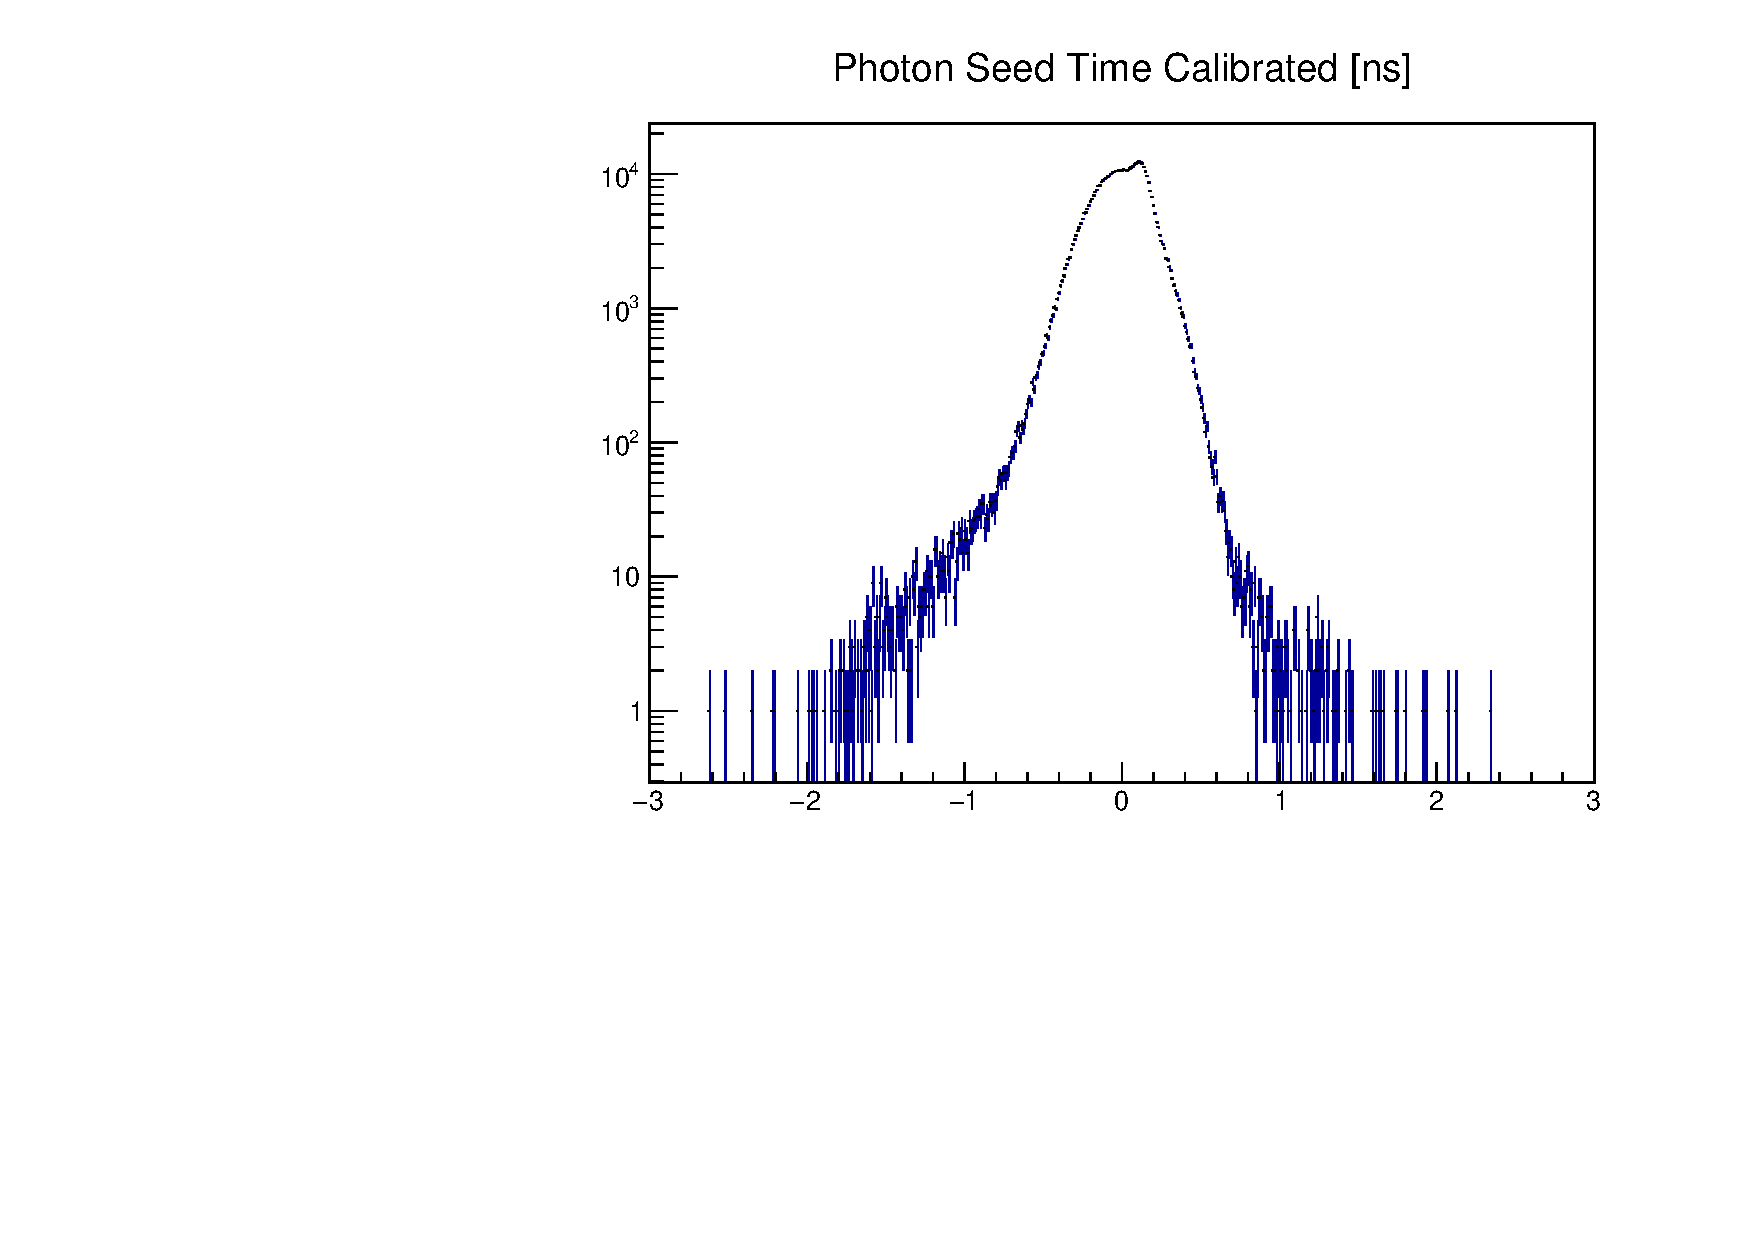
\includegraphics{fig/sec_algos/cc_dist_v24_18A_316241_316457.pdf}}
%\caption{  ..  place holder for plot of CC skim distro and 2D dt vs effA plot  ...}
%\label{ccdistros}
%\end{center}
%\end{figure}


